
\documentclass[12pt,a4paper]{book}



			% Packages Files
%----------------------------------%

	% Page Setttings
\usepackage[top = 1in, bottom = 1in, left = 1in, right = 1in]{geometry}

\parindent=0cm % to prevent the spacing in new paragraph or new line

\usepackage{fancyhdr} % needded for header and footer 

%-----------------------------------------------------------------%

\usepackage{amsmath} % needed for referencing thequation
\usepackage{amsfonts} % for maths symbols
\usepackage{graphicx}
\usepackage[export]{adjustbox}
\usepackage{caption}
\usepackage{refstyle} % to reference a captioned figure


% To make hyperlinks

\usepackage[
	colorlinks=true
	,breaklinks
	]{hyperref} % needed for creating hyperlinks in the document, the option colorlinks=true gets rid of the awful boxes, breaklinks breaks lonkg links (list of figures),
	
\usepackage{xcolor}
\definecolor{c1}{rgb}{0,0,1} % blue
\definecolor{c2}{rgb}{0,0.3,0.9} % light blue
\definecolor{c3}{rgb}{0.3,0,0.9} % red blue
\hypersetup{
    linkcolor={c1}, % internal links
    citecolor={c2}, % citations
    urlcolor={c3} % external links/urls
}

	% For Code Writing
	
\usepackage{listings}

\usepackage{color}

\definecolor{mygreen}{rgb}{0 0.6 0}

\lstset{
% Set automatic Line breaking, in case we have long lines don't
% fit inside the frame or the page.
breaklines = true,
commentstyle = \color{mygreen},
breakatwhitespace = true,% don't show white space character
%numbers = left, % put line number in the code
title = \lstname
}

% ------------- For Writing Equations inisde a table and centering them ------------

\usepackage{array}

% Vertical Alignment inside the cells of the table
\newcolumntype{M}[1]{>{\centering\arraybackslash}m{#1}}

% Horizontal Alignment inside the cells of the table
\newcolumntype{P}[1]{>{\centering\arraybackslash}p{#1}}


% needed for todos liste
\usepackage{todonotes} 


\usepackage{nomencl}



% Macros File

% Macros Example
\def\labelaxes{Remember to include some suitable labeling for the axes and the units used in measurements.}

% 2nd way for defnining macros: the new command
% 1st parameter: name of the new command
% 2nd paramter: how many inputs this command needs, in this case only 1
% 3rd parameter: what this new command named \tbi do

\newcommand{\tbi}[1]{\textbf{\textit{#1}}}

% Command for Picture without a label

\newcommand{\pic}[3]{\begin{figure}[h]
\centering
\includegraphics[width = 0.7\textwidth, frame]{#1}
\caption{#2}
\end{figure}}






\DeclareMathOperator*{\argmax}{argmax} % thin space, limits underneath in displays

\DeclareMathOperator*{\argmin}{argmin}

\title{Compressed Sensing}
\author{Ranim Tom}



\begin{document}


\maketitle

\tableofcontents

\pagestyle{fancy}
\fancyhf{} % Clear header and footer
\rhead{\rightmark}
\lhead{Chapter \thechapter}
\rfoot{Page \thepage}


\chapter{Compressed Sensing}

\underline{Source:} Lecture by Prof Michael Lusting, Berkeley University.\\


\section{Introduction and Motivation}

\begin{itemize}

\item Usually when we store information (images captured by camera, some audio files, $\cdots$), we store them in a compressed way, as shown in \autoref{fig:Compressed_Sensing:MRI}

\begin{figure}[h]
\centering
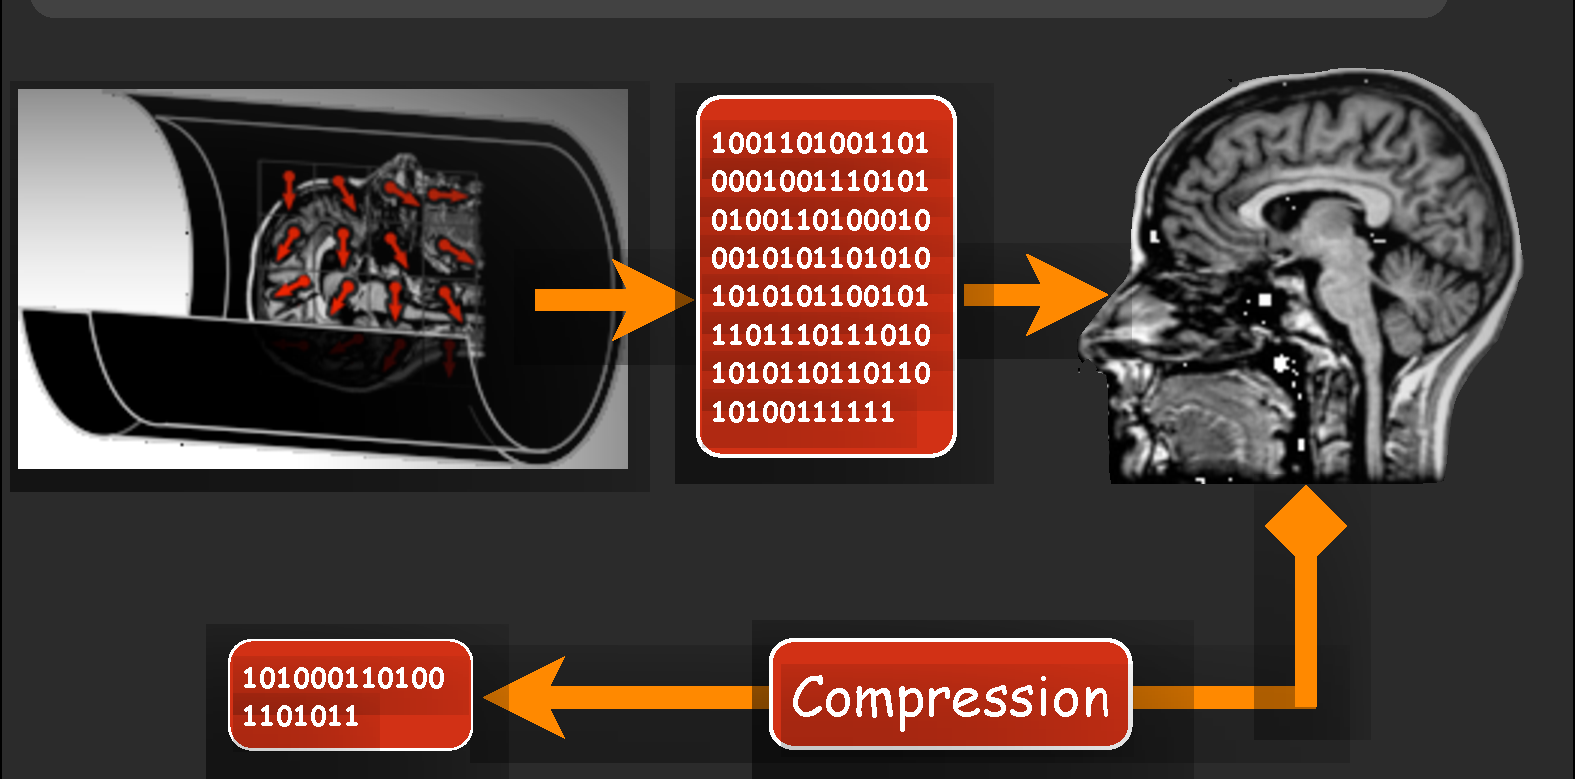
\includegraphics[width = 0.7\textwidth, frame]{Figures/Compressed_Sensing/MRI.pdf}
\caption{Compressing MRI: first we collect, then we compress}
\label{fig:Compressed_Sensing:MRI}
\end{figure}

	\begin{itemize}
	\item In other words, depending on \autoref{fig:Compressed_Sensing:MRI}, we usually spend allot of time constructing the data (the measurements), construct the image (the MRI), then inputted to compression algorithm to compress it and \tbi{throw away allot of measurements we spend time to collect them !}.
	
	\end{itemize}


\item As a side note for compression: we usually compress data depending on human perception (hearing or seeing), in such a way we restore only valuable information (so not all the data) and we can't see or hear (in case of audio) the difference 

\newpage
\item But what if \tbi{we can sense directly} the information, as shown in \autoref{fig:Compressed_Sensing:MRI}

\begin{figure}[h]
\centering
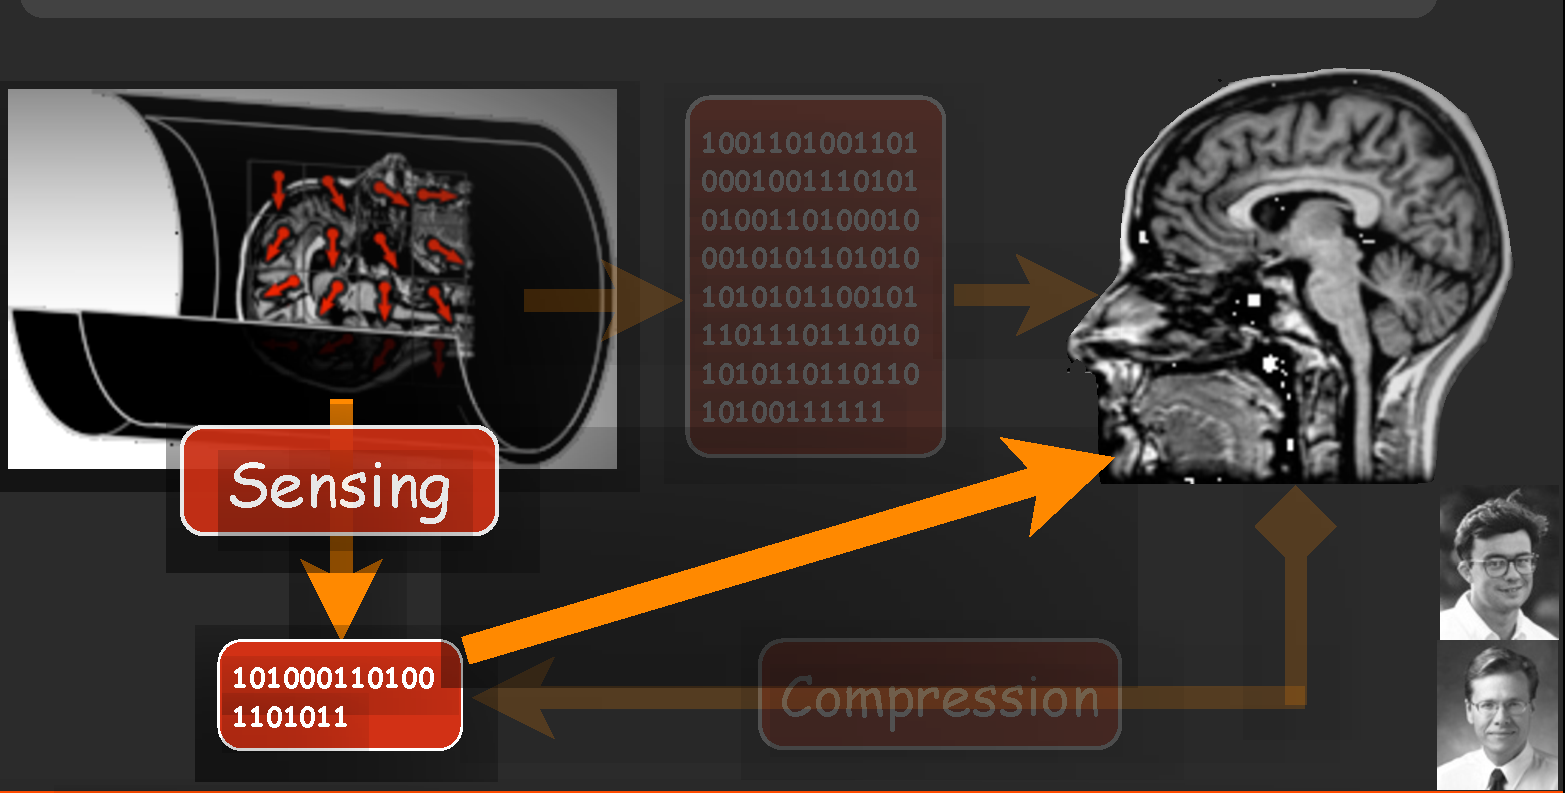
\includegraphics[width = 0.7\textwidth, frame]{Figures/Compressed_Sensing/MRI_Sensing}
\caption{Sensing Concept}
\label{fig:Compressed_Sensing:MRI_Sensing}
\end{figure}

The approach shown in \autoref{fig:Compressed_Sensing:MRI} is very helpful because by this way, we don't need to throw allot of information we gathered as in \autoref{fig:Compressed_Sensing:MRI}, and directly collect the valuable information needed for reconstruction.


\end{itemize}

\section{Example of Compression and Interpretation}

\begin{itemize}

\item First let's see some audio signal in \autoref{fig:Compressed_Sensing:Audio}

\begin{figure}[h]
\centering
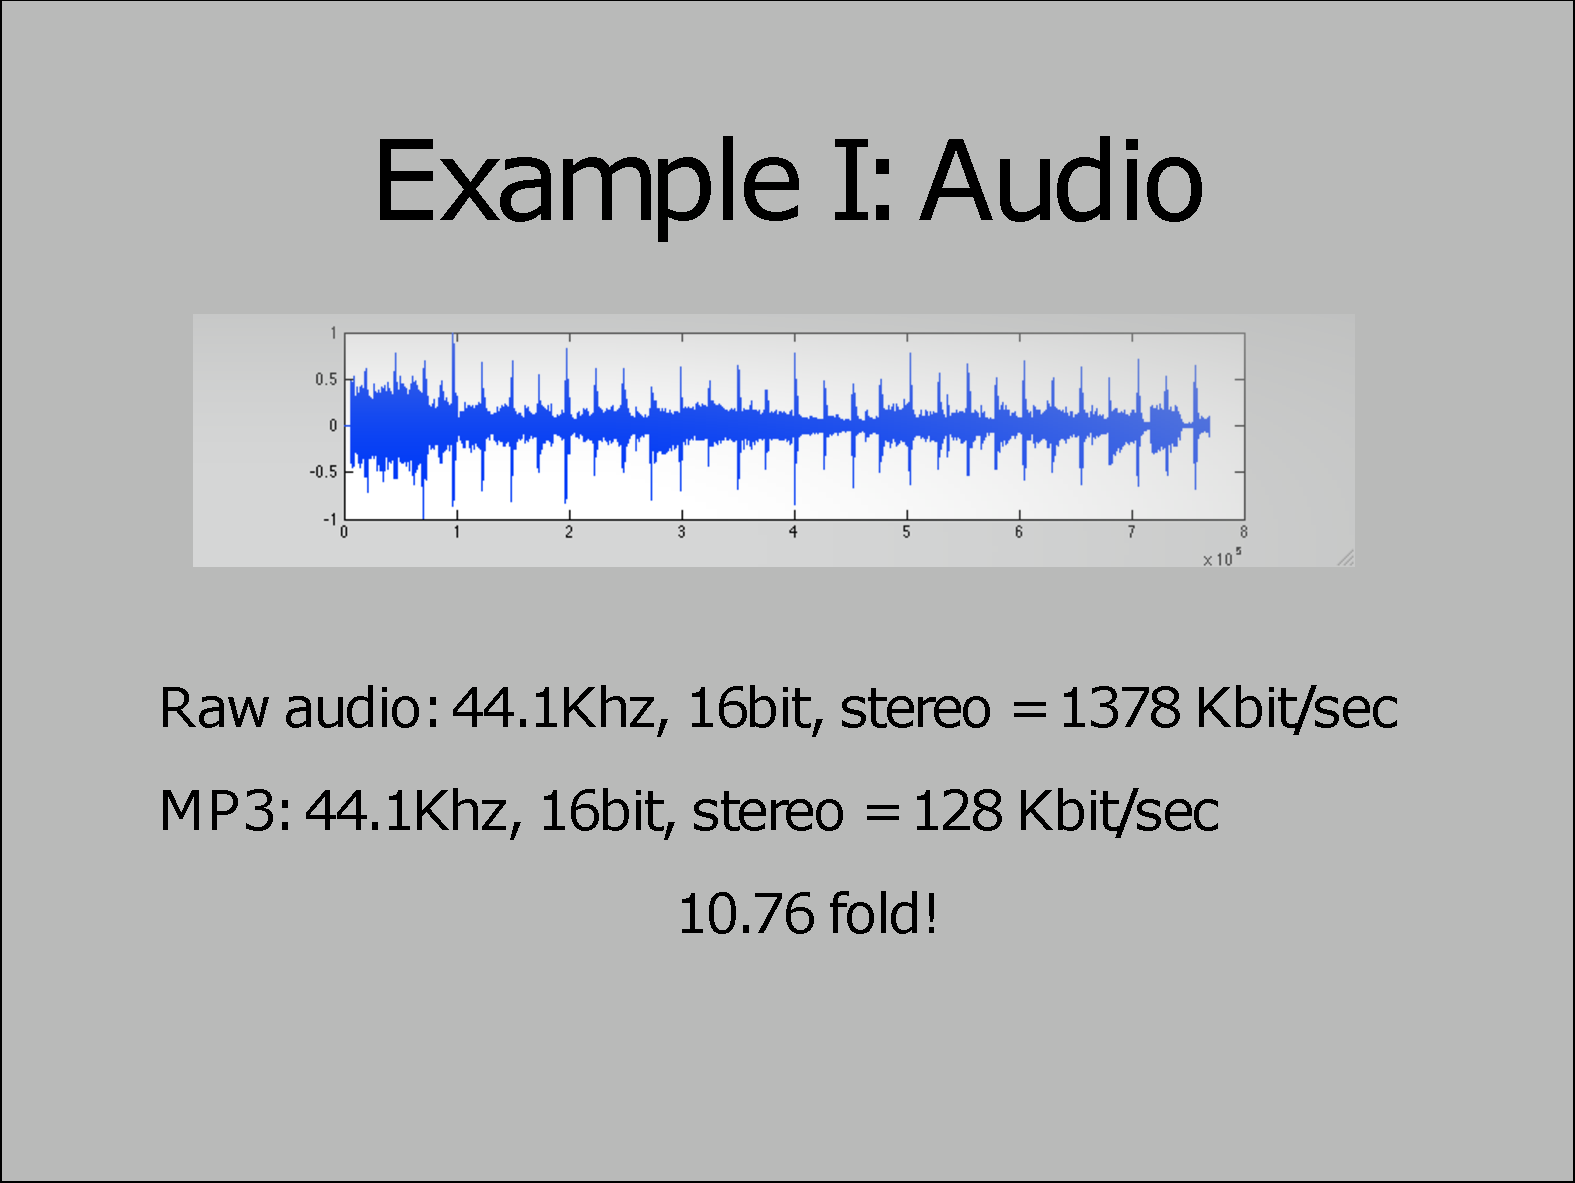
\includegraphics[width = 0.7\textwidth, frame]{Figures/Compressed_Sensing/Audio}
\caption{Audio Compression}
\label{fig:Compressed_Sensing:Audio}
\end{figure}

	\begin{itemize}
	
	\item As interpretation, if we listen at a rate of 128 Kbit/s, it would make no difference if we here in original rate
		
	\end{itemize}


\item What about images ? are images compressible like audio.

Images are generally more complex type of signals, because they are higher in dimension.

An example is shown in \autoref{fig:Compressed_Sensing:Image}.


\begin{figure}[h]
\centering
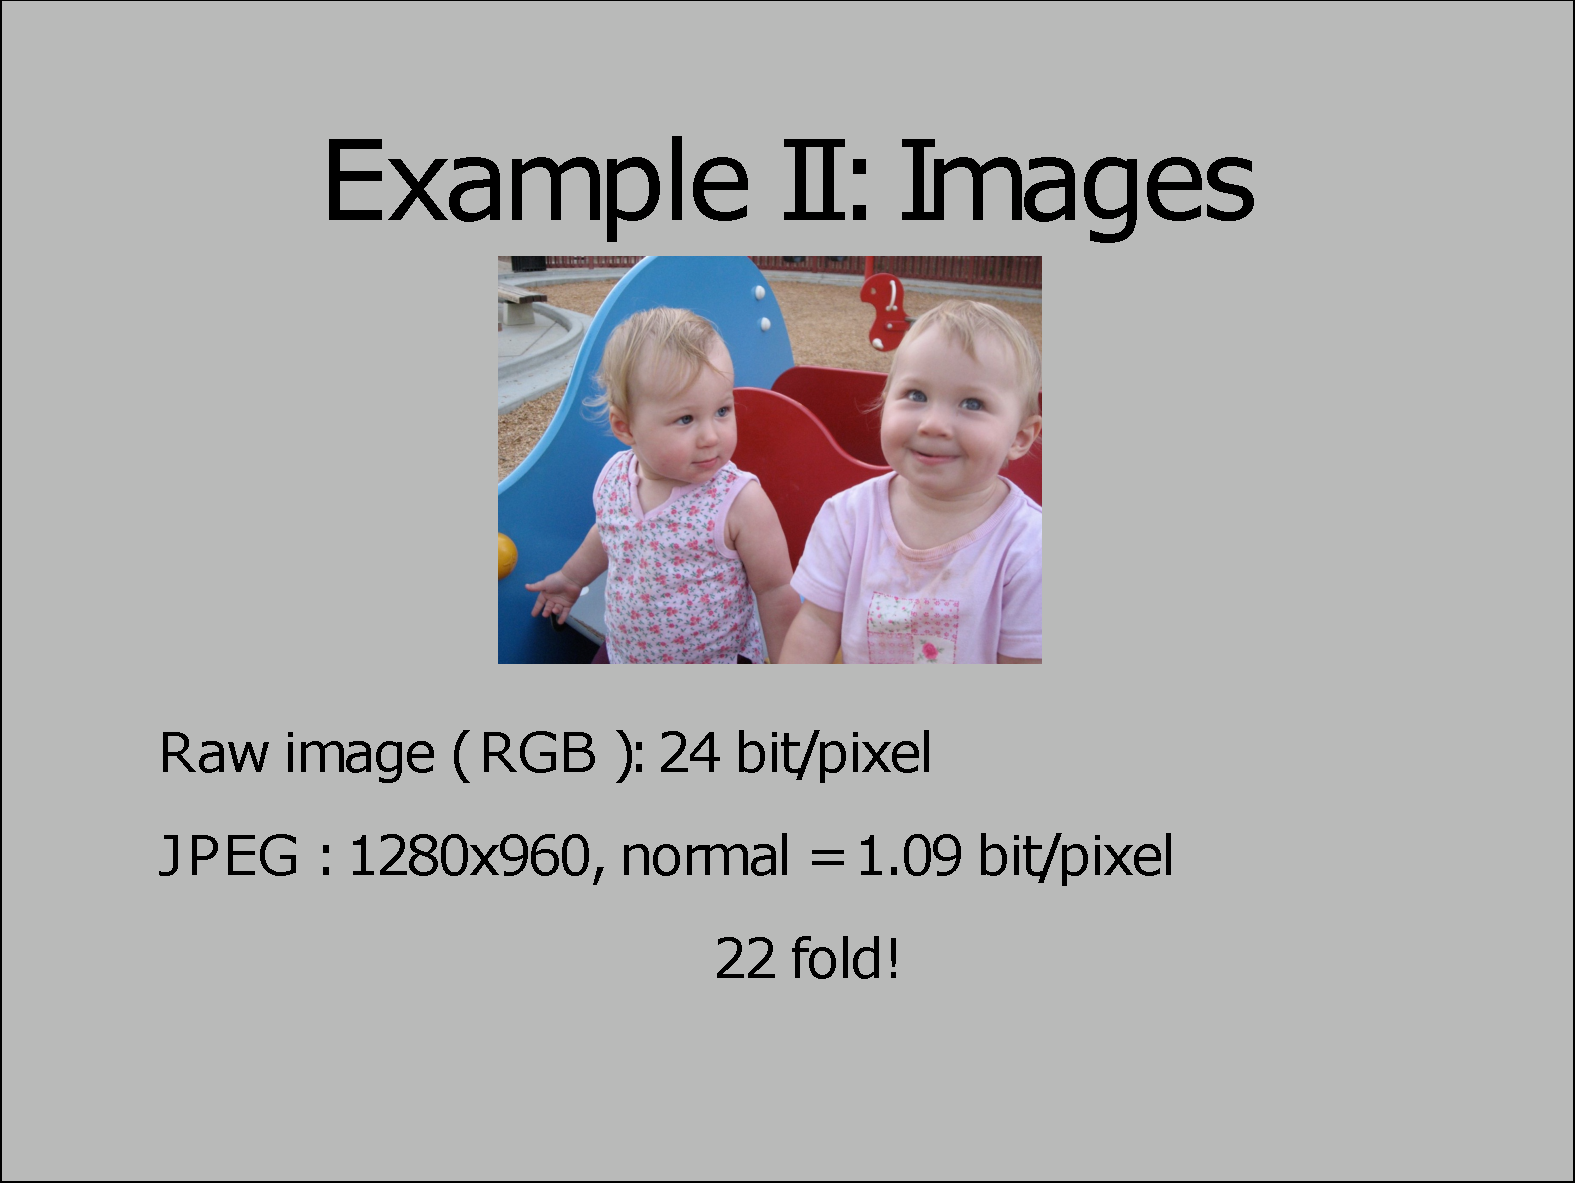
\includegraphics[width = 0.7\textwidth, frame]{Figures/Compressed_Sensing/Image}
\caption{Image Compression}
\label{fig:Compressed_Sensing:Image}
\end{figure}


	\begin{itemize}
	\item It turns out that we can compress with higher compression ration
	
	\item It is true that dimension increase, but the information doesn't necessary increase also as the dimension (power of 2 in this casee)
	
	\item The thing is there is allot of correlation we can use in the channel 
	\end{itemize}


\newpage
\item Same concept applied to video signals, shown in \autoref{fig:Compressed_Sensing:Video}.

\begin{figure}[h]
\centering
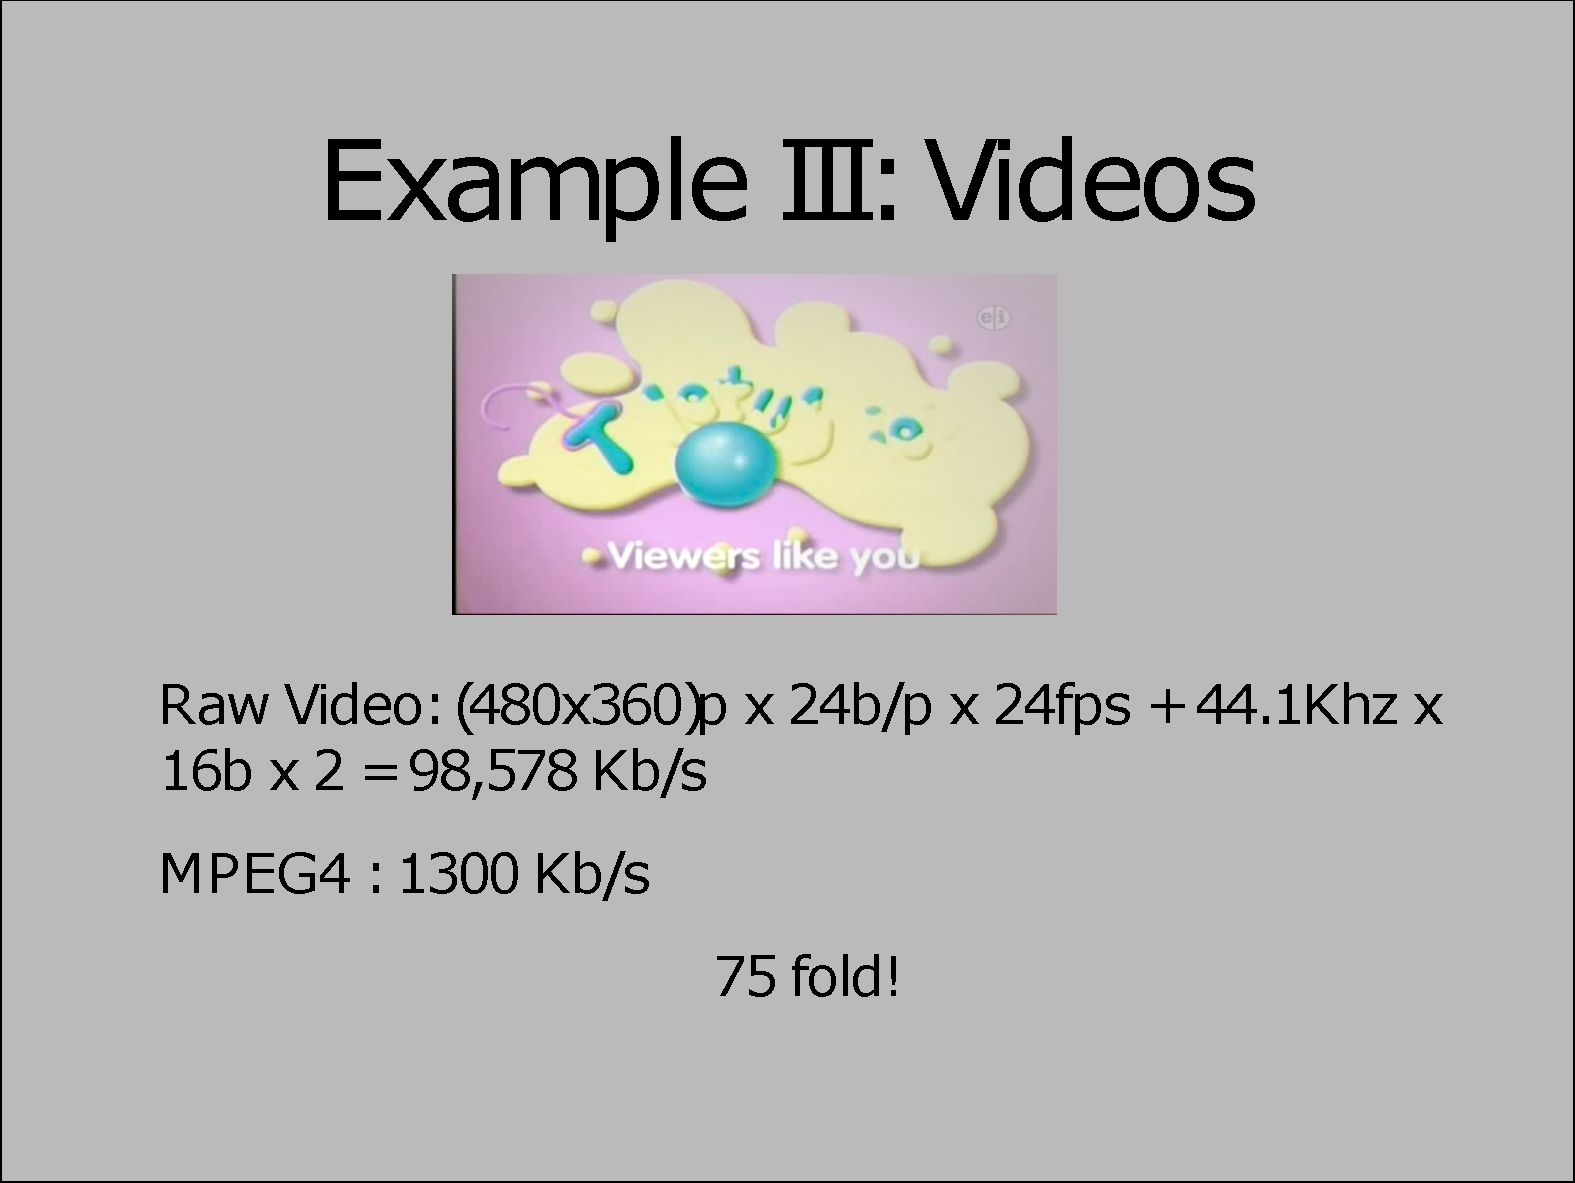
\includegraphics[width = 0.7\textwidth, frame]{Figures/Compressed_Sensing/Video}
\caption{Video Compression}
\label{fig:Compressed_Sensing:Video}
\end{figure}


\end{itemize}

\newpage
\section{Steps of Compression}

General steps of compression are shown in \autoref{fig:Compressed_Sensing:Compression_steps}.

\begin{figure}[h]
\centering
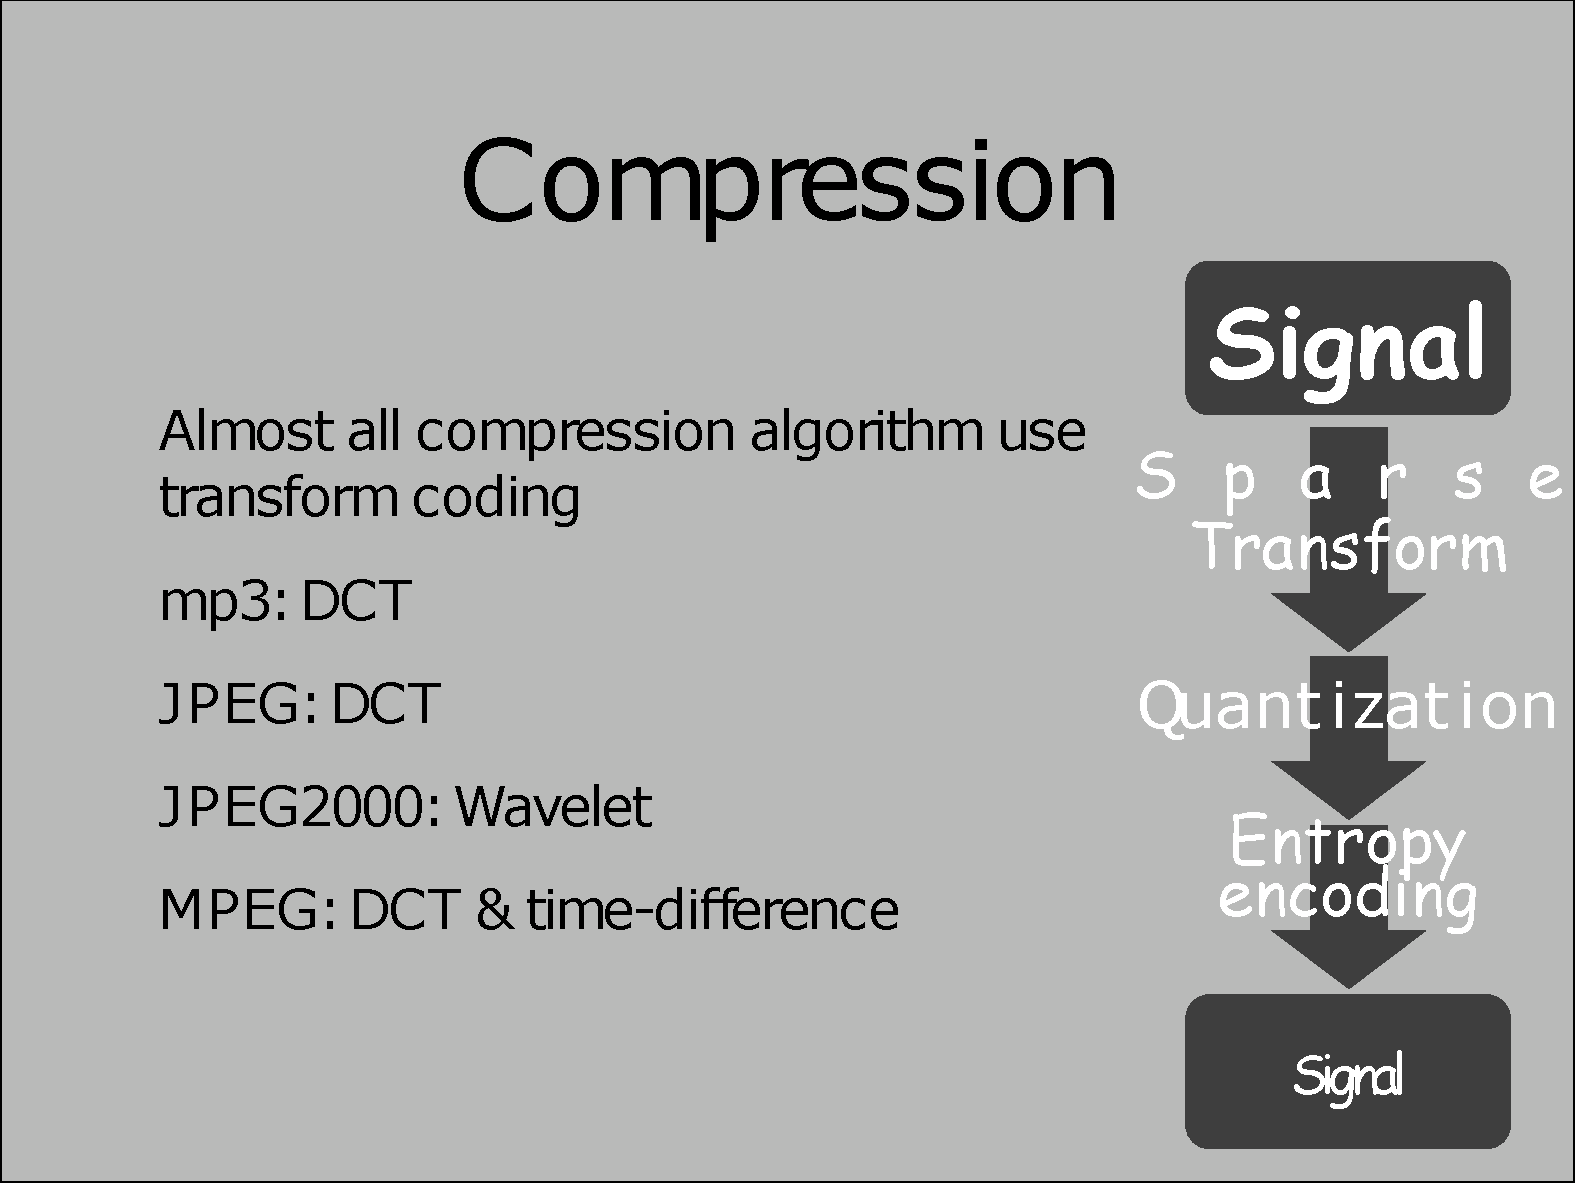
\includegraphics[width = 0.7\textwidth, frame]{Figures/Compressed_Sensing/Compression_steps}
\caption{Compression Steps}
\label{fig:Compressed_Sensing:Compression_steps}
\end{figure}

\begin{itemize}

\item We apply some sparse transformation

	\begin{itemize}
	\item Sparse transformation decompose the signals in some set of few coefficients
	\end{itemize}


\item We quantize these coefficients and do some entropy coding

\end{itemize}

\newpage
\section{Sparsity and Noise}

Usually, when we have a sparse signal with noise, we can identify the signal directly by simple threshold operation. So in other words, sparse signals (or sparse representation in some other domains) have the ability to separate between the useful components of the signals (non zero component with large values usually) and with noisy components which tends to have small values. This is actually known as denoising by using sparsity. These concepts are illustrated in \autoref{fig:Compressed_Sensing:Sparsity_Noise}.


\begin{figure}[h]
\centering
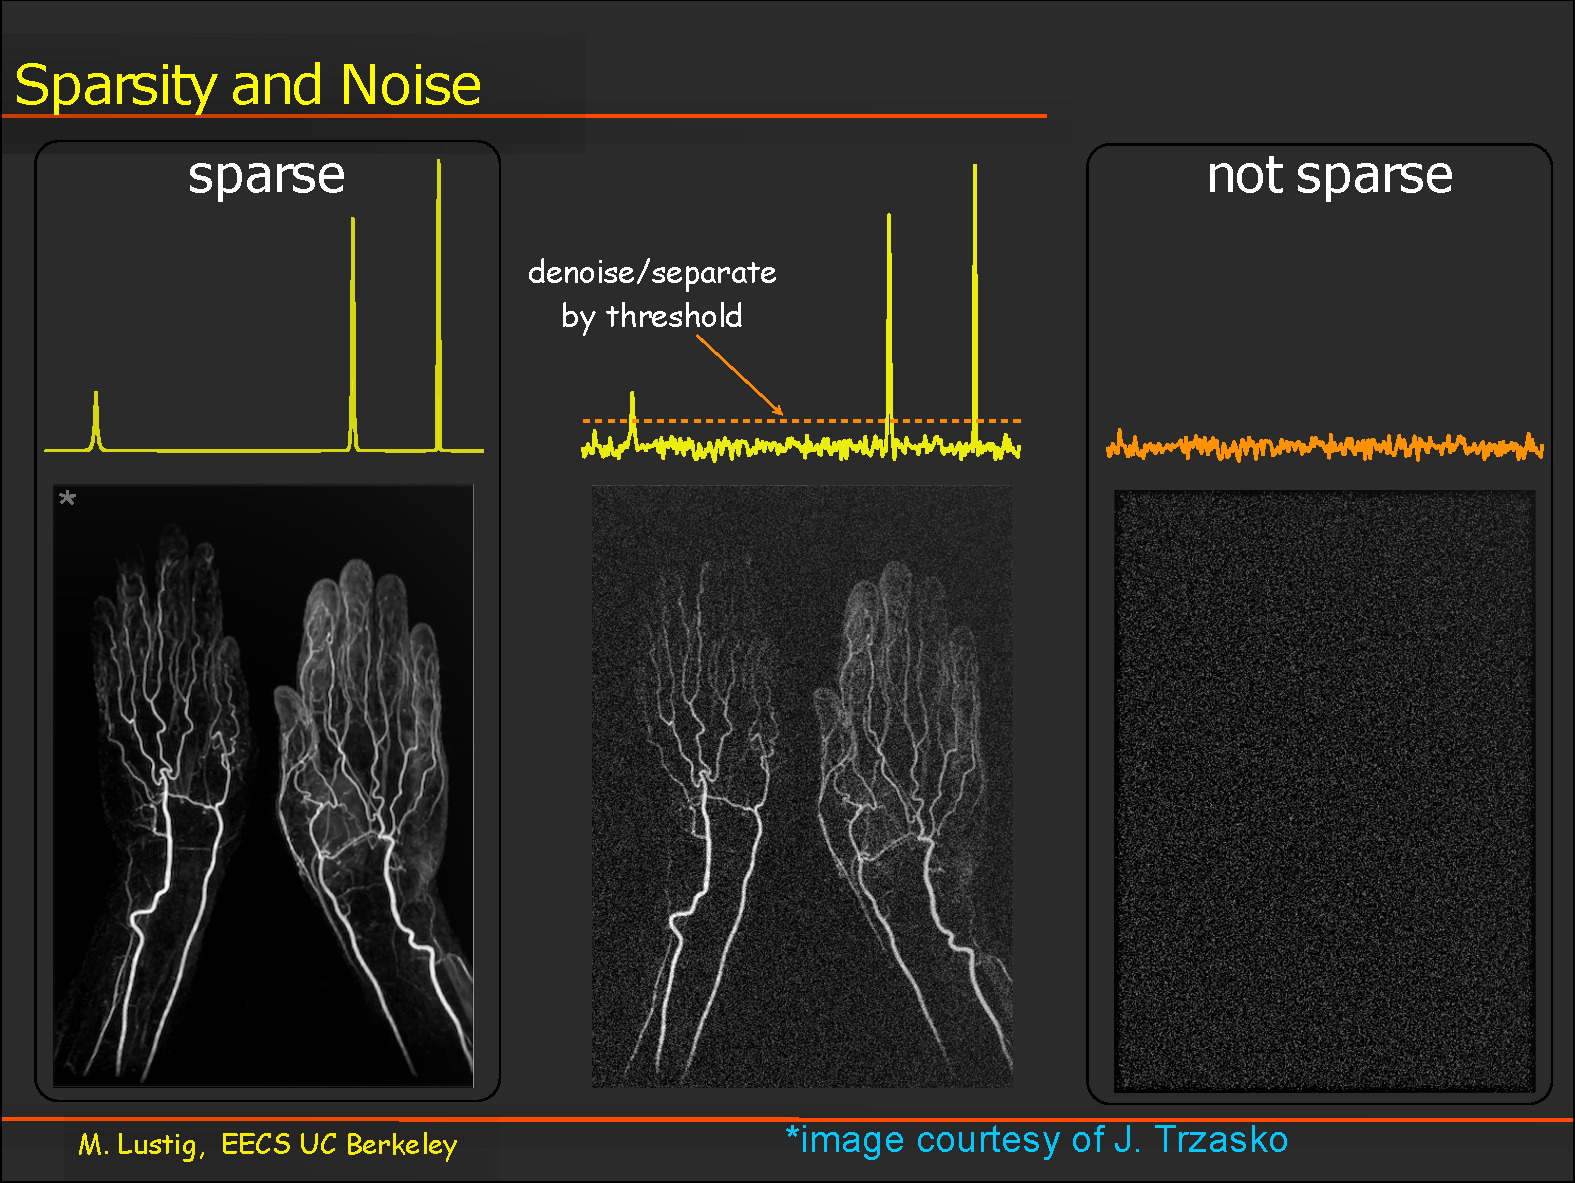
\includegraphics[width = 0.7\textwidth, frame]{Figures/Compressed_Sensing/Sparsity_Noise}
\caption{Noise Reduction taking advantage from sparse nature of signal}
\label{fig:Compressed_Sensing:Sparsity_Noise}
\end{figure}


\newpage
Some example of brain image using wavelet decomposition shown in \autoref{fig:Compressed_Sensing:brain_wavelet}

\begin{figure}[h]
\centering
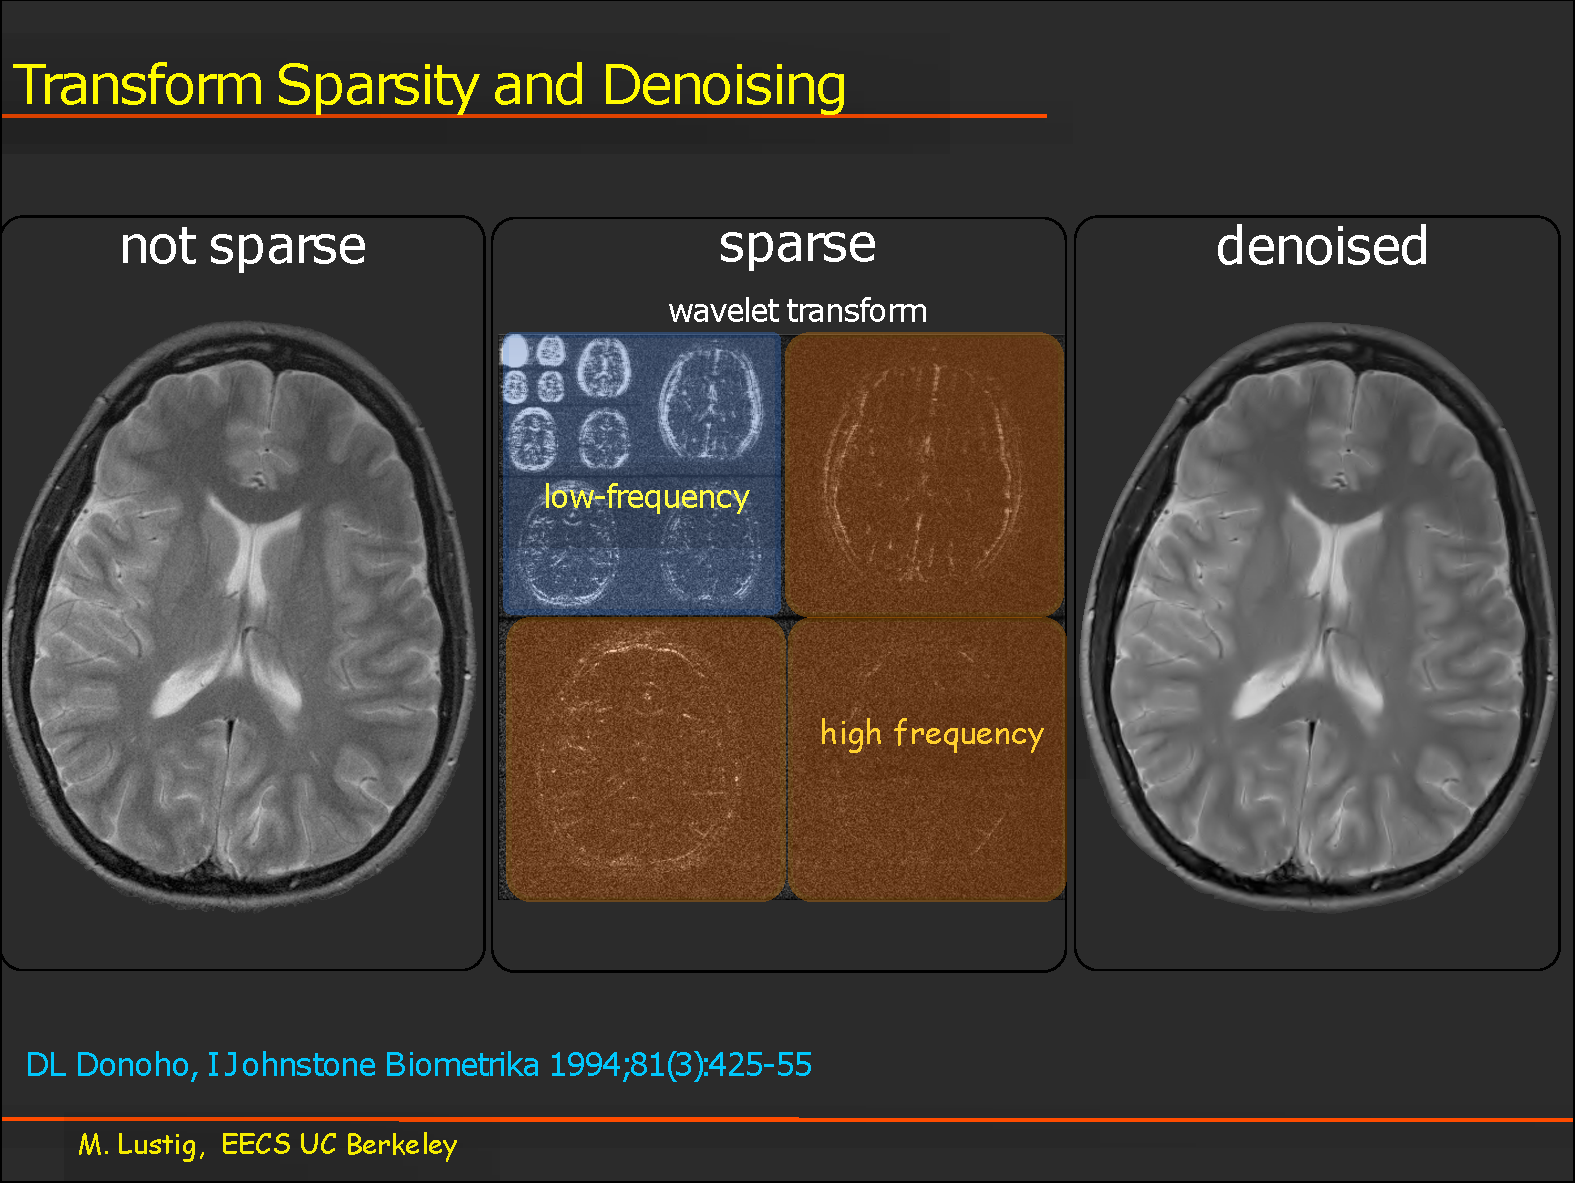
\includegraphics[width = 0.7\textwidth, frame]{Figures/Compressed_Sensing/brain_wavelet}
\caption{Noise Reduction using wavelet transform}
\label{fig:Compressed_Sensing:brain_wavelet}
\end{figure}


\begin{itemize}

\item It is true that the image is not sparse. However its wavelet decomposition is sparse and hence we can use thresholding to reduce the noise level and reconstruct the image


\end{itemize}


\newpage
\section{Moving to Compressive Sampling}

We have seen in sections before that sparsity help us with noise reduction and compression, but we didn't see its relation with compressive sampling, yet !.\\

Let's see the concepts of compressive sampling shown in \autoref{fig:Compressed_Sensing:compressive_sampling_concept} 

\begin{figure}[h]
\centering
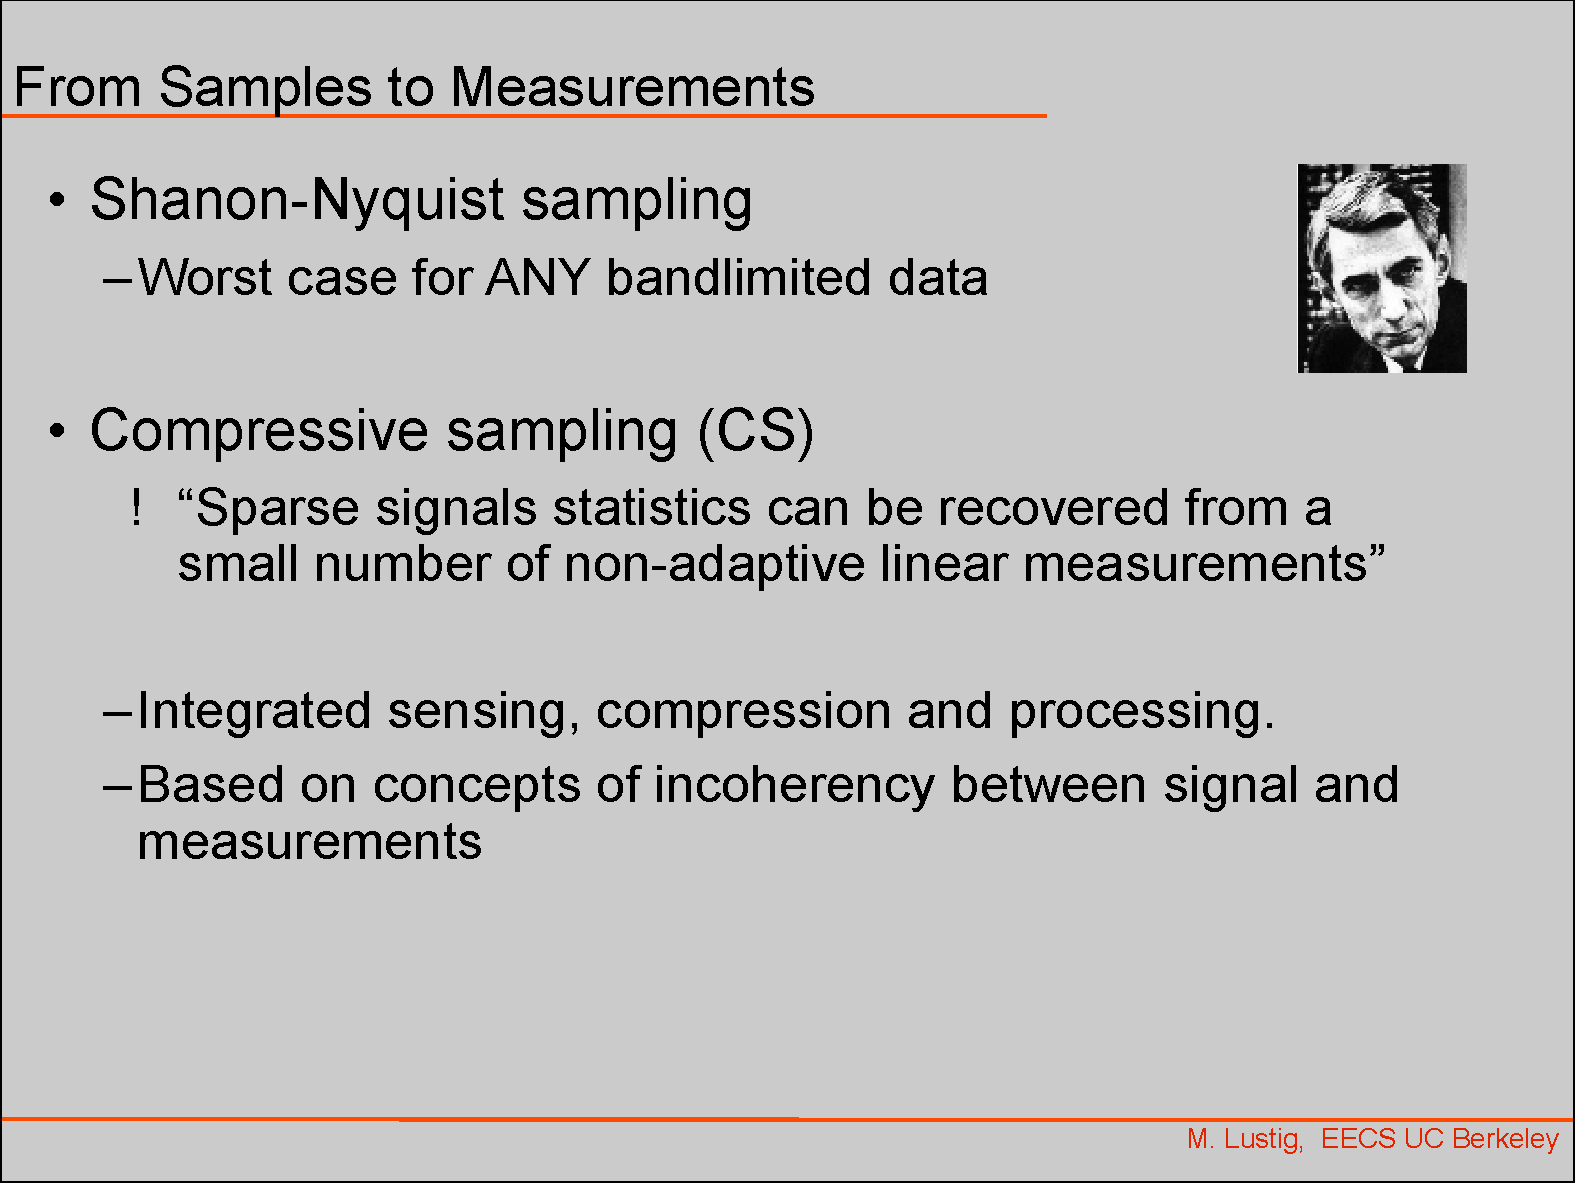
\includegraphics[width = 0.7\textwidth, frame]{Figures/Compressed_Sensing/compressive_sampling_concept}
\caption{Compressive Sampling Concept}
\label{fig:Compressed_Sensing:compressive_sampling_concept}
\end{figure}

\begin{itemize}

\item Usually by following Nyquist theorem, we can  reconstruct the full signal

\item However in compressive sampling, we reduce the number of samples and still able to do reconstruction

\end{itemize}

\newpage
Let's begin first by the \tbi{classical sensing} case, shown in \autoref{fig:Compressed_Sensing:classical_sensing}

\begin{figure}[h]
\centering
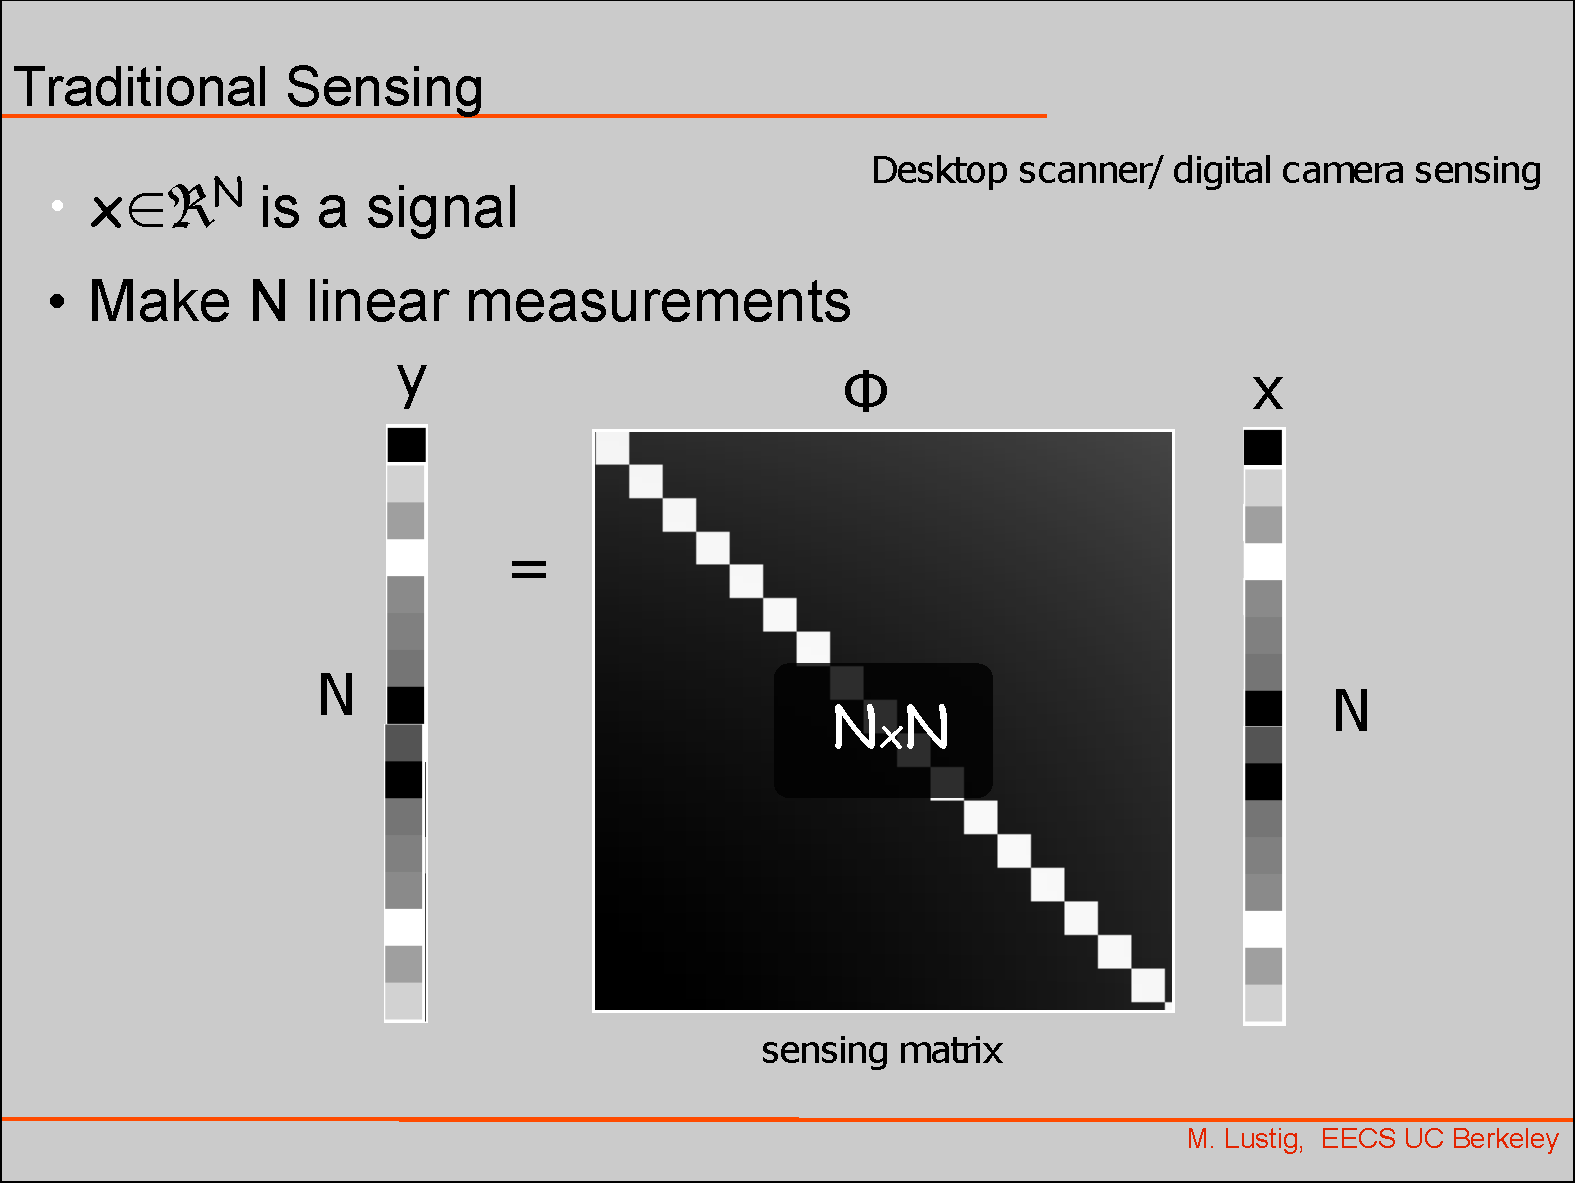
\includegraphics[width = 0.7\textwidth, frame]{Figures/Compressed_Sensing/classical_sensing}
\caption{Classical Sensing Concept}
\label{fig:Compressed_Sensing:classical_sensing}
\end{figure}

\begin{itemize}

\item We have some signal $x \,\in \mathbb{R}^N$ and we need to recover it

\item What we can do is to construct some $N$ independent linear measurement vector $y$ using a sensing matrix $\Phi$

	\begin{itemize}
	\item The matrix $\Phi$ shown in \autoref{fig:Compressed_Sensing:classical_sensing} is an identity matrix related to single pixel camera experiment
	\end{itemize}


\newpage
\item The best sensing matrix is the orthogonal matrix: $\Phi \, \times \, \Phi^T \, = \, \text{I}$

	\begin{itemize}
	\item Any orthogonal matrix can be used as a sensing matrix. Another example of sensing matrix $\Phi$ is shown in \autoref{fig:Compressed_Sensing:classical_sensing_FFT}, where it is the FFT matrix used in MRI
	
	
\begin{figure}[h]
\centering
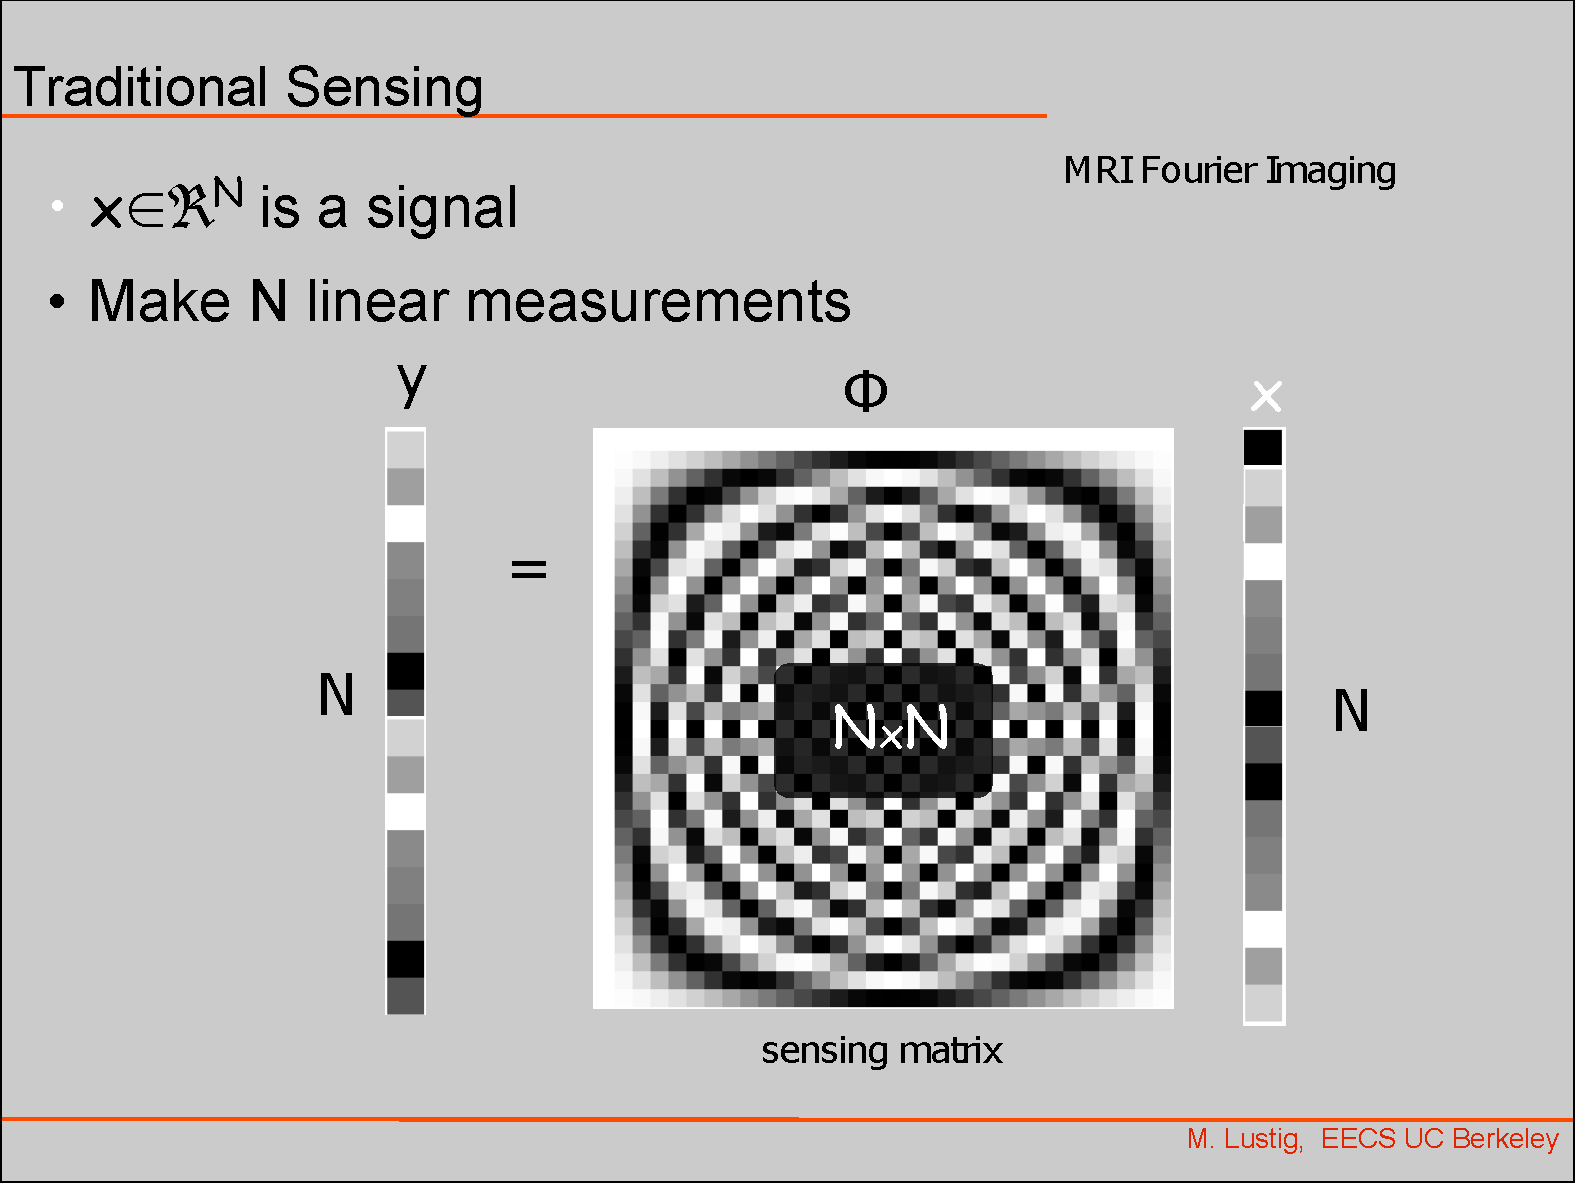
\includegraphics[width = 0.7\textwidth, frame]{Figures/Compressed_Sensing/classical_sensing_FFT}
\caption{Classical Sensing: FFT matrix in MRI}
\label{fig:Compressed_Sensing:classical_sensing_FFT}
\end{figure}
	
	
	\end{itemize}


\end{itemize}


So the classical case for estimating some unknown vector $x \,\in \mathbb{R}^N$, is to take the same number $N$ on liner independent measurement.\\

Now let's shift the gears to the sparse case shown in \autoref{fig:Compressed_Sensing:sparse_sensing}.
	
\begin{figure}[h]
\centering
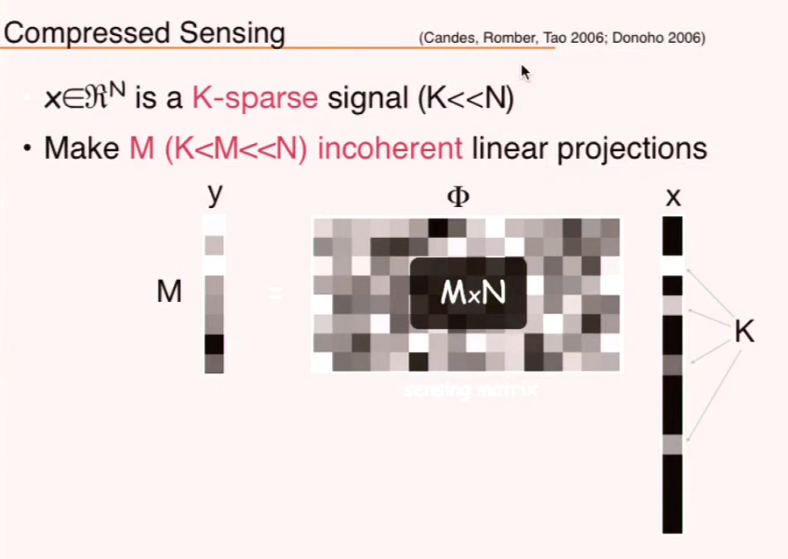
\includegraphics[width = 0.7\textwidth, frame]{Figures/Compressed_Sensing/sparse_sensing}
\caption{Sparse Sensing}
\label{fig:Compressed_Sensing:sparse_sensing}
\end{figure}

\begin{itemize}

\item If my signal $x$ is sparse, then we don't need to do $N$ linear independent measurement

	\begin{itemize}
	\item What we do is take $M$ measurements such that $M$ is far less than $N$, and little big than $K$, $\rightarrow \, K \, < \, M \, << \, N$
	\end{itemize}

\item In the case of sparse also, the sensing matrix $\Phi$ becomes flat (rectangular), so it will not become fully orthogonal, but approximately orthogonal

	\begin{itemize}
	\item What approximately orthogonal means that the columns of $\Phi$ will try to be orthogonal as much as they can
	
	\item And also the product $\Phi \, \times \, \Phi^T$ will give an approximate identity matrix, where the elements off the diagonal tends to 0, but not exactly 0
	
\begin{figure}[h]
\centering
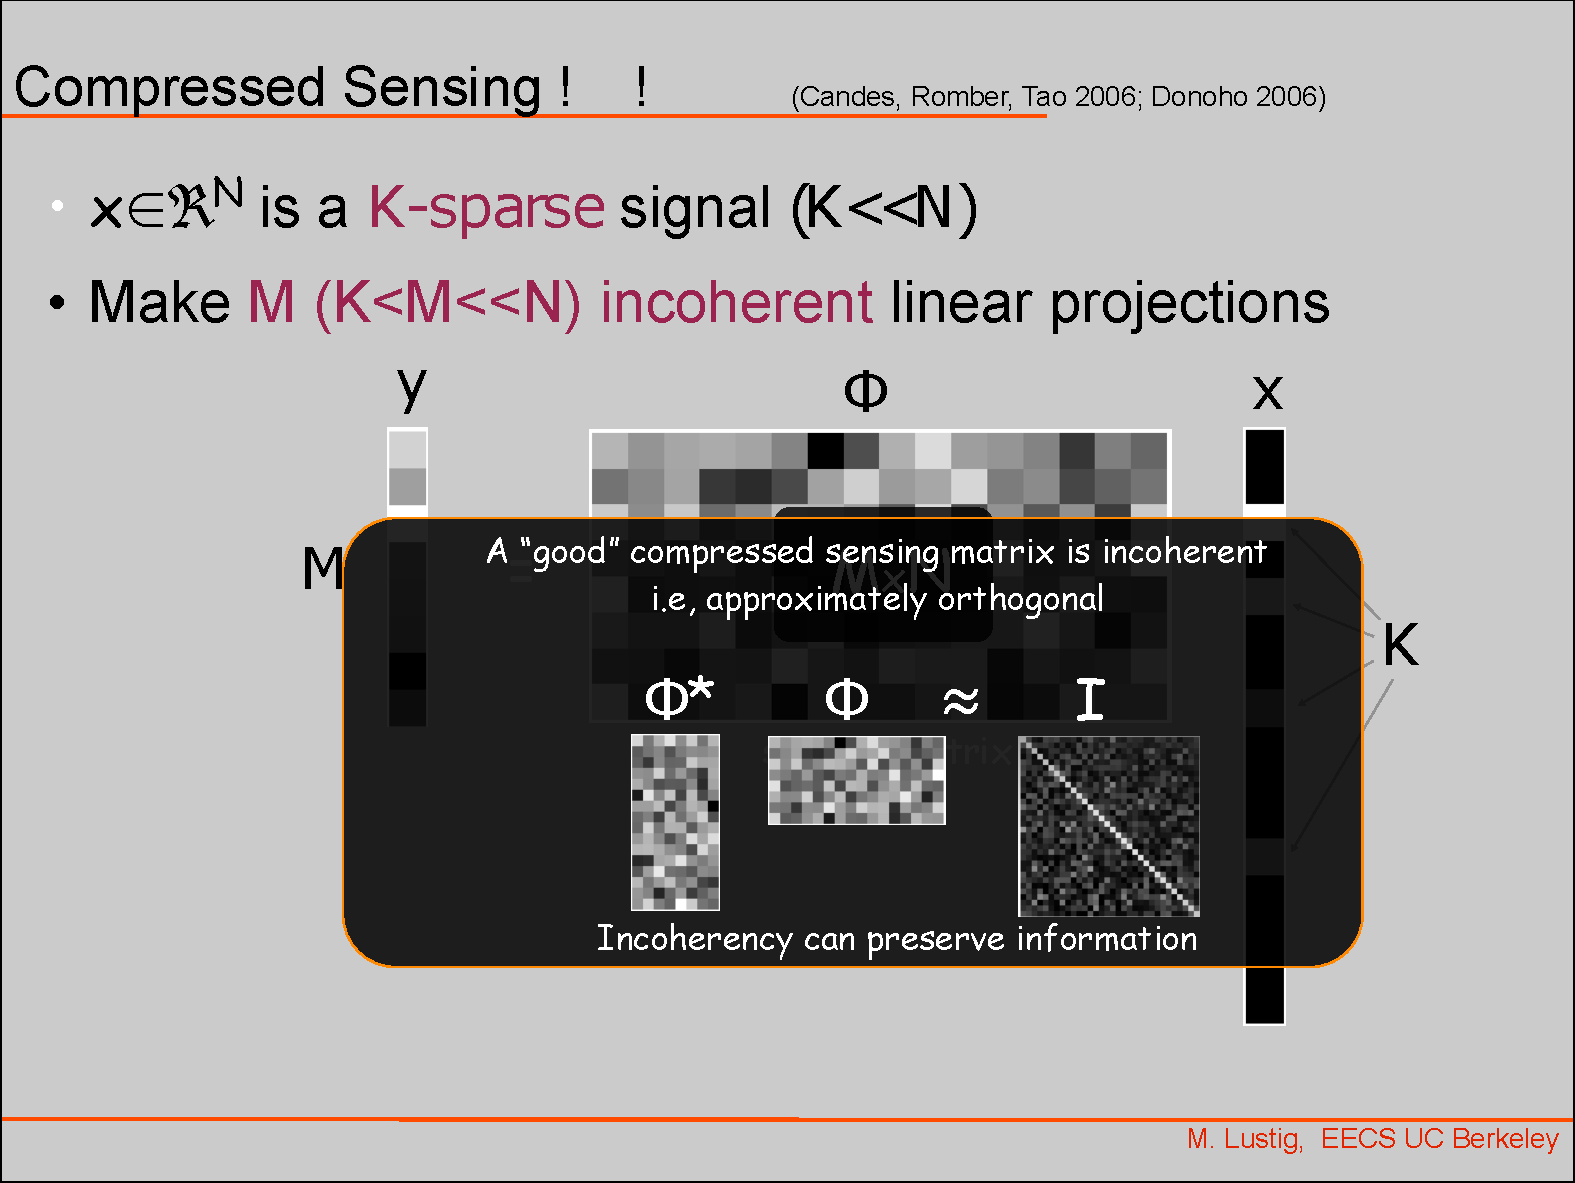
\includegraphics[width = 0.7\textwidth, frame]{Figures/Compressed_Sensing/sparse_sensing_matrix}
\caption{Sparse Sensing matrix $\Phi$}
\label{fig:Compressed_Sensing:sparse_sensing_matrix}
\end{figure}	
	

	\end{itemize}

\end{itemize}

If we look again at \autoref{fig:Compressed_Sensing:sparse_sensing}, we can do the following:

\begin{itemize}

\item If we know where the non zero coefficient are in $x$, so we can recover $x$ by eliminating the unnecessary columns in $\Phi$ which multiply the 0 elements

\item In relation with band limited signals, we know where our frequency content is concentrated (the analogy with location of non zero components in signal $x$), so we can design some sampling criteria lower than the Nyquist rate in which we can recover the signal with no aliasing

\end{itemize}

However, we usually don't know where these non zero values are, so that's a problem.\\

However, we can benefit from the constraint that $x$ is sparse, and try to formulate it in some optimization formulation. There are many ways to try:

\begin{itemize}

\item Some natural intuition is because $x$ is sparse, we can try to minimize the energy subject to $y \, = \, \Phi \, x$, which can be written as: 


\begin{equation}
\begin{array}{rcl}
\min \parallel x \parallel_2 \\
\text{s.t } y \, = \, \Phi \, x
\end{array}
\end{equation}

\end{itemize}



\chapter{Compressed Sensing 2: Dr Steve Brunton}

\section{References}

Read chapter 3 in \cite{data_driven_approach}.

\section{Notes}

\begin{itemize}

\item A sparse representation: $x_{N \times 1} \, = \, \Psi_{N \times N} \, \times \, s_{N \times 1}$

 where $\begin{cases}
s \text{ is a sparse vector} \\
x \text{ is the natural signal in the intial domain (time or spatial)}
\end{cases}$

\item Even if we compress and we are able to return $x$ from $x$, the compresses sensing framework let us choose only few measurements and restore $s$.

\begin{figure}[h]
\centering
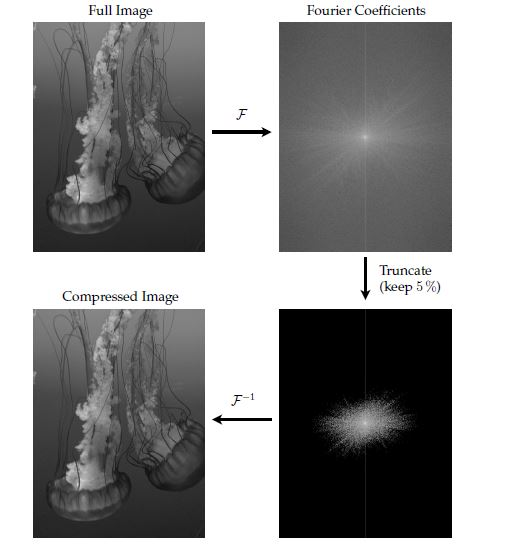
\includegraphics[width = 0.7\textwidth, frame]{Figures/Compressed_Sensing/Compression_Fourier}
\caption{Compression using Fourier Basis}
\label{fig:Compressed_Sensing:Compression_Fourier}
\end{figure}
 
\newpage 
\item However, in compression, we are making many measurements then throwing away most of these values

	\begin{itemize}
	\item So what if we can directly make few measurements, recover the sparse vector $s$, then take the inverse Fourier to restore the original signal $x$
	
	
	\item Mathematically, this can be done:
	
	\begin{equation}
	\begin{array}{rcl}
	y_{m \times 1} \, &=& \, C_{m \, \times \, N} \,\times \,  x_{N \times 1} \\ 
		 &=& \, C_{m \, \times \, N} \, \times \, \Psi_{N \times N} \, \times \, s_{N \times 1} \\
		 &=& \, \Theta \, \times \, s_{N \times 1}

	\end{array}
	\label{Eq:Compressed_Sensing:formulation_2}
	\end{equation}
	
	
\end{itemize}	 

\item \underline{Mathematics:}

	\begin{itemize}
	\item The system of equation by (\ref{Eq:Compressed_Sensing:formulation_2}) is known to be an undertimined system 
	
		\begin{itemize}
		\item There are infinite number of $s$ vectors which satisfy equation (\ref{Eq:Compressed_Sensing:formulation_2})
		\end{itemize}
		
	\item However, we know that $s$ should be sparse (a constraint which we need to satisfy), hence we add a regularization term to the objective function	
	
		\begin{itemize}
		\item This the work of many genius people in the field of optimization, statistics and programming
		\end{itemize}

\item For many years, people have used the $\ell_2 ~$ norm 

	\begin{itemize}
	\item $\ell_2 ~$  norm doesn't produce a sparse solution
	
	\item It minimize the radius of the circle (the energy) but all the component of the signal (vector) are still active
	\end{itemize}

\begin{figure}[h]
\centering
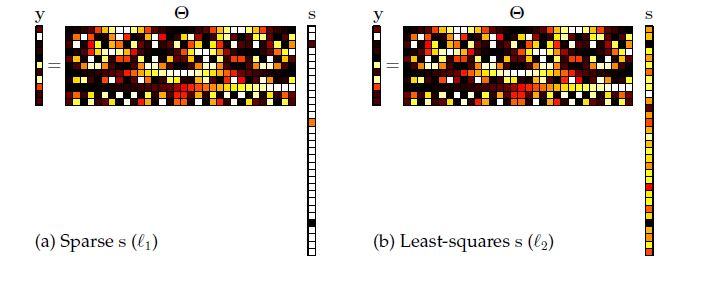
\includegraphics[width = 0.7\textwidth, frame]{Figures/Compressed_Sensing/l1_l2_norms_differences}
\caption{$\ell_1 ~$ and $\ell_2 ~$ norms effects}
\label{fig:Compressed_Sensing:norms_effect}
\end{figure}

\item \underline{Objective Function writing for this problem:} 

\begin{equation}
\begin{array}{rcl}
\text{min }  ||\, C_{m \, \times \, N} \, \times \, \Psi_{N \times N} \, \times \, s_{N \times 1} \, - \, y \,||_2 \, + \, \lambda \, || s||_1
\end{array}
\label{Eq:Compressed_Sensing:formulation_optimization_1}
\end{equation}
	
Or we can formulate it as in (\ref{Eq:Compressed_Sensing:formulation_optimization_2}):

\begin{equation}
\begin{array}{rcl}
\min ||\, s \, ||_1 \text{ subject to }  || \, C_{m \, \times \, N} \, \times \, \Psi_{N \times N} \, \times \, s_{N \times 1} \, - \, y \, ||_2 \, \leq \, \epsilon
\end{array}
\label{Eq:Compressed_Sensing:formulation_optimization_2}
\end{equation}	

where $\epsilon$ is a tolerance we set due to some noise in the measurement
		
	\end{itemize}


 

\end{itemize}

\section{Conditions}

Recalling the matrix formulation:

	\begin{equation}
	\begin{array}{rcl}
	y_{m \times 1} \, &=& \, C_{m \, \times \, N} \,\times \,  x_{N \times 1} \\ 
		 &=& \, C_{m \, \times \, N} \, \times \, \Psi_{N \times N} \, \times \, s_{N \times 1} \\
		 &=& \, \Theta \, \times \, s_{N \times 1}

	\end{array}
	\label{Eq:Compressed_Sensing:formulation_2_recall}
	\end{equation}

In order to solve the optimization problem, we need to be aware of several conditions to be respect:

\begin{itemize}

\item $C$ is called the measurement matrix, where is has to satisfy some conditions

	\begin{enumerate}
	\item Incoherence with respect to $\Psi$: $C$ needs not be parallel 
	
	\item Good measurement matrices can be Gaussian distributed, Bernoulli,$\cdots$.
	
	So they are random. Put picture here. 
	
	\item A bad measurement matrix example: if we take $\Psi^T$.
	
	If we do so, we won't capture all the frequencies (or features) of the sparse vector $s$. Put the picture here.
	
	\item \underline{Note}: it is usually that mathematicians love Gaussian distributed matrices because they are robust mathematically. However, this not usually true in engineering problems. For example, the single pixel camera measurement matrix is used often (to do this later)
	\end{enumerate}


\item Number of measurements $p$ : they have to be $	\propto O \left(\, k \, \text{log}\displaystyle \left(\,\frac{n}{k}  \,\right)\,\right)$
\end{itemize}


%**************** References ****************

\bibliographystyle{IEEEtran}

\bibliography{Literature/Books_Signal_Processing,Literature/Papers_Signal_Processing}


\end{document}

